\documentclass[letter,12pt]{article}
\usepackage[letterpaper,right=1in,left=1in,top=1in,bottom=1in]{geometry}
\usepackage{setspace}

\usepackage[utf8]{inputenc}   % allows input of special characters from keyboard (input encoding)
\usepackage[T1]{fontenc}      % what fonts to use when printing characters       (output encoding)
\usepackage{amsmath}          % facilitates writing math formulas and improves the typographical quality of their output
\usepackage[hyphens]{url}     % adds line breaks to long urls
\usepackage[pdftex]{graphicx} % enhanced support for graphics
\usepackage{tikz}             % Easier syntax to draw pgf files (invokes pgf automatically)
\usetikzlibrary{arrows}

\usepackage{mathptmx}           % set font type to Times
\usepackage[scaled=.90]{helvet} % set font type to Times (Helvetica for some special characters)
\usepackage{courier}            % set font type to Times (Courier for other special characters)

\usepackage[longnamesfirst, sort]{natbib}\bibpunct[]{(}{)}{,}{a}{}{;} % handles biblio and references 

\usepackage{rotating}         % sideway tables and figures that take a full page
\usepackage{caption}          % allows multipage figures and tables with same caption (\ContinuedFloat)

\usepackage{dcolumn}          % needed for apsrtable and stargazer tables from R to compile
\usepackage{arydshln}         % dashed lines in tables (hdashline, cdashline{3-4}, 
                              %see http://tex.stackexchange.com/questions/20140/can-a-table-include-a-horizontal-dashed-line)
                              % must be loaded AFTER dcolumn, 
                              %see http://tex.stackexchange.com/questions/12672/which-tabular-packages-do-which-tasks-and-which-packages-conflict


\newcommand{\mc}{\multicolumn}

%% TO ADD NOTES IN TEXT, PUT % BEFORE THE ONE YOU WANT DISABLED
\usepackage[disable]{todonotes}                            % no show
%\usepackage[colorinlistoftodos, textsize=small]{todonotes} % show notes
\newcommand{\emm}[1]{\todo[color=red!15, inline]{\textbf{Eric:} #1}}

%% \usepackage{xr} % allows cross-ref to other file
%% \externaldocument{urge15appendix}

%% %for submission: sends figs, tables, and footnotes to last pages
%% \RequirePackage[nomarkers,nolists]{endfloat}     % sends tables and figures to the end
%% \RequirePackage{endnotes}                        % turns fn into endnotes; place \listofendnotes where you want 
%%                                                  %the endnotes to appear (it must be after the last endnote).
%% \let\footnote=\endnote
%% \newcommand{\listofendnotes}{
%%    \begingroup
%%    \parindent 0pt
%%    \parskip 2ex
%%    \def\enotesize{\normalsize}
%%    \theendnotes
%%    \endgroup
%% }

%% % for submission: drop page numbers when producing title page
%% \pagenumbering{gobble} % Remove page numbers (and reset to 1)
%% \pagenumbering{arabic}% Arabic page numbers (and reset to 1)


\setcitestyle{citesep={;}}

\begin{document}

\title{Incumbency advantage upon removal of single-term limits: Mexican municipal elections}
\author{Eric Magar \\ ITAM, Mexico City
}
\date{\today}
\maketitle

% \newpage

\begin{abstract}
\noindent En route
%% \newline
%% \newline
%% \textbf{Keywords}: Separation of Powers, Urgency Prerrogatives, Fast Track Authority, Legislative Process, Latin America, Chile
\end{abstract}

% \newpage

%\doublespacing

\section{Introduction}

\noindent En route

\section{A hypothesis perhaps}

\begin{figure}
  \centering
    \caption{The president rules game}\label{F:game}
    \tikzstyle{mid}=[circle,draw]
    \begin{tikzpicture}
      \node[mid] at (1.5,-0.25) (c) {\emph{C}};
      \node[mid] at (4,1) (p) {\emph{P}};
      \node[mid] at (6.5,-0.25) (f) {\emph{F}};
      \node at (4,-1.5) (ce) {$q$};
      \node at (6.5,2.25) (pe1) {$x_F$};
      \node at (9,1) (fe1) {$x_C$};
      \node at (9,-1.5) (fe2) {$q$};
      \path[-] (c) edge node [above, sloped] {\footnotesize{report}} (p)
               (p) edge node [above, sloped] {\footnotesize{fast}} (f)
                   edge node [below, sloped] {\footnotesize{track}} (f);
      \path[] (c) edge node [below, sloped] {\footnotesize{$x_C$}} (p);
      \path[-o] (c) edge node [below, sloped] {\footnotesize{not}} (ce)
                (p) edge node [above, sloped] {\footnotesize{standard}} (pe1)
                (f) edge node [above, sloped] {\footnotesize{accept}} (fe1)
                    edge node [below, sloped] {\footnotesize{reject}} (fe2);
      \path[-o] (p) edge node [below, sloped] {\footnotesize{considerat.}} (pe1);
    \end{tikzpicture}
\end{figure}

\begin{description}
  \item [Hypothesis 1:] Presidents are more likely to fast-track bills when the committee chair with jurisdiction over the bill  belongs to the president's party than otherwise.
\end{description}

\section{Incumbents running v.\ open seats}

\begin{tabular}{l|cccc|cccc}
        &   \mc{4}{c|}{incumbent on the ballot}    &      \mc{4}{c}{open seat}          \\
In party& \%won   & \%lost   &   sum   &     (N)  & \%won  & \%lost &   sum   &      (N)\\ \hline
pan     &   66    &   34     &   100   &   (121)  &   39   &   61   &   100   &   (1663)\\
pri     &   49    &   51     &   100   &   (219)  &   50   &   50   &   100   &   (3546)\\
prd     &   55    &   45     &   100   &    (88)  &   39   &   61   &   100   &   (1082)\\
morena  &  100    &    0     &   100   &     (8)  &   88   &   12   &   100   &     (18)\\
other   &   45    &   55     &   100   &    (99)  &   25   &   75   &   100   &    (631)\\ \hline
total   &   54    &   46     &   100   &   (535)  &   44   &   56   &   100   &   (6940)\\
\end{tabular}

\begin{tabular}{lcccccccc}
        &   \mc{4}{c}{incumbent on the ballot}    &      \mc{4}{c}{open seat, party}   \\
In party&   won   &   lost   &   sum   &   (N)    &   won  &   lost &   sum   &   (N)\\
left    &   58    &   42     &   100   &   (96)   &   39   &   61   &   100   &   (1100)\\
\end{tabular}

\section{Regression model}

% Table created by stargazer v.5.2.2 by Marek Hlavac, Harvard University. E-mail: hlavac at fas.harvard.edu
% Date and time: Tue, Sep 29, 2020 - 05:17:38 PM
% Requires LaTeX packages: dcolumn 
\begin{table}[!htbp] \centering 
  \caption{} 
  \label{} 
\begin{tabular}{@{\extracolsep{5pt}}lD{.}{.}{-3} D{.}{.}{-3} D{.}{.}{-3} } 
\\[-1.8ex]\hline 
\hline \\[-1.8ex] 
 & \multicolumn{3}{c}{\textit{Dependent variable:}} \\ 
\cline{2-4} 
\\[-1.8ex] & \multicolumn{3}{c}{Residual} \\ 
 & \multicolumn{1}{c}{PAN} & \multicolumn{1}{c}{PRI} & \multicolumn{1}{c}{Left} \\ 
\\[-1.8ex] & \multicolumn{1}{c}{(1)} & \multicolumn{1}{c}{(2)} & \multicolumn{1}{c}{(3)}\\ 
\hline \\[-1.8ex] 
 vote share (lagged) & -0.187^{***} & -0.035^{***} & -0.339^{***} \\ 
  & (0.011) & (0.013) & (0.013) \\ 
  & & & \\ 
 party incumbent & 0.224^{***} & 0.171^{***} & 0.165^{***} \\ 
  & (0.013) & (0.014) & (0.018) \\ 
  & & & \\ 
 other-party incumbent & -0.021^{**} & -0.011 & 0.005 \\ 
  & (0.010) & (0.009) & (0.010) \\ 
  & & & \\ 
 party open seat & 0.162^{***} & 0.124^{***} & 0.130^{***} \\ 
  & (0.004) & (0.004) & (0.005) \\ 
  & & & \\ 
 governor & -0.009^{*} & 0.028^{***} & 0.008 \\ 
  & (0.005) & (0.004) & (0.006) \\ 
  & & & \\ 
 population (10k) & 0.002 & 0.002^{**} & 0.006^{***} \\ 
  & (0.001) & (0.001) & (0.001) \\ 
  & & & \\ 
 elevation (pop. weigthed) & -0.003 & -0.00005 & -0.031^{***} \\ 
  & (0.003) & (0.003) & (0.003) \\ 
  & & & \\ 
 sd.elev & -0.143^{***} & -0.038 & -0.080^{**} \\ 
  & (0.034) & (0.031) & (0.035) \\ 
  & & & \\ 
 post reform & 0.085^{***} & -0.156^{***} & 0.047^{***} \\ 
  & (0.005) & (0.005) & (0.006) \\ 
  & & & \\ 
 elev x sd.elev & 0.105^{***} & -0.017 & 0.085^{***} \\ 
  & (0.024) & (0.022) & (0.025) \\ 
  & & & \\ 
 Intercept & -0.041^{***} & -0.036^{***} & -0.062^{***} \\ 
  & (0.005) & (0.007) & (0.004) \\ 
  & & & \\ 
\hline \\[-1.8ex] 
Observations & \multicolumn{1}{c}{8,314} & \multicolumn{1}{c}{8,314} & \multicolumn{1}{c}{8,314} \\ 
R$^{2}$ & \multicolumn{1}{c}{0.213} & \multicolumn{1}{c}{0.293} & \multicolumn{1}{c}{0.183} \\ 
%Adjusted R$^{2}$ & \multicolumn{1}{c}{0.212} & \multicolumn{1}{c}{0.292} & \multicolumn{1}{c}{0.182} \\ 
Residual Std. Error (df = 8303) & \multicolumn{1}{c}{0.163} & \multicolumn{1}{c}{0.152} & \multicolumn{1}{c}{0.169} \\ 
F Statistic (df = 10; 8303) & \multicolumn{1}{c}{225.2$^{***}$} & \multicolumn{1}{c}{344.3$^{***}$} & \multicolumn{1}{c}{185.6$^{***}$} \\ 
\hline 
\hline \\[-1.8ex] 
\textit{Note:}  & \multicolumn{3}{r}{$^{*}$p$<$0.1; $^{**}$p$<$0.05; $^{***}$p$<$0.01} \\ 
\end{tabular} 
\end{table} 


\section{Discussion}

\begin{figure}
  \centering
    \caption{Population-weigthed altitude deviations in municipalities}\label{F:avgMg}
    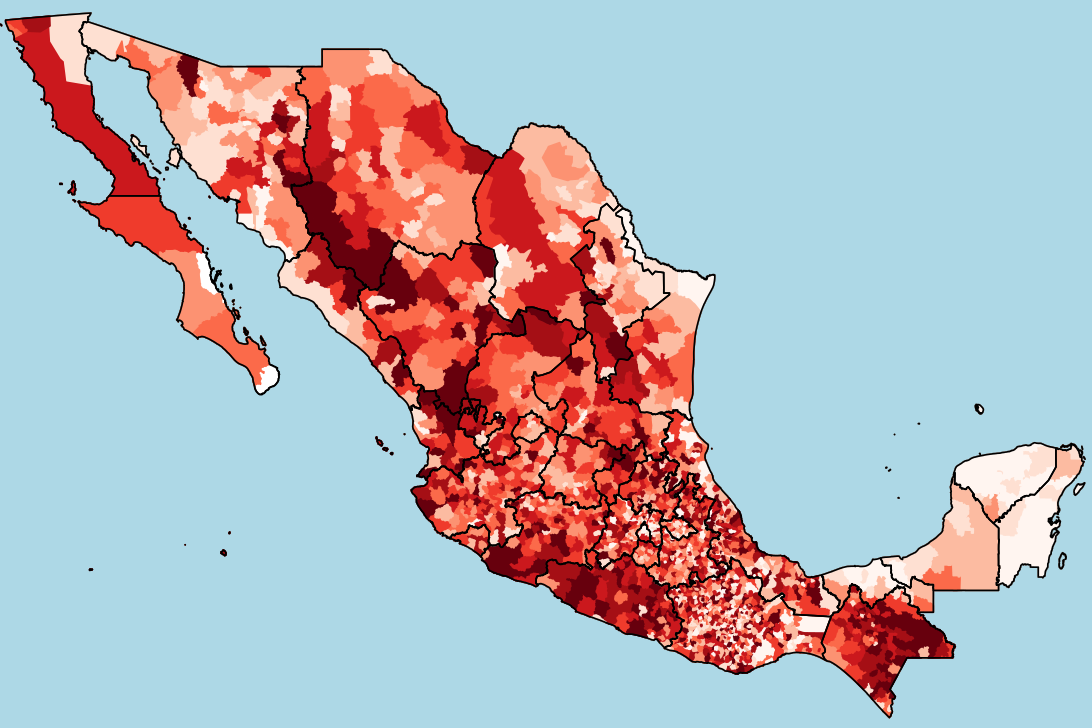
\includegraphics[width=.8\columnwidth]{../graph/map.png}
\end{figure}


\section*{Acknowledgements}
The author received financial support from the Asociaci\'on Mexicana de Cultura \textsc{a.c.}\ and \textsc{conacyt}'s Sistema Nacional de Investigadores. He is responsible for mistakes and shortcomings in the study.

%% \listofendnotes

\bibliographystyle{apsr}
\bibliography{../bib/magar}

\end{document}

